\documentclass{sig-alternate}




% Use this command to override the default ACM copyright statement (e.g. for preprints).
% Consult the conference website for the camera-ready copyright statement.


%% EXAMPLE BEGIN -- HOW TO OVERRIDE THE DEFAULT COPYRIGHT STRIP -- (July 22, 2013 - Paul Baumann)
 %\toappear{Permission to make digital or hard copies of all or part of this work for personal or classroom use is 	granted without fee provided that copies are not made or distributed for profit or commercial advantage and that copies bear this notice and the full citation on the first page. Copyrights for components of this work owned by others than ACM must be honored. Abstracting with credit is permitted. To copy otherwise, or republish, to post on servers or to redistribute to lists, requires prior specific permission and/or a fee. Request permissions from permissions@acm.org. \\
% {\emph{BuildSys'16}}, Nov 16--17, 2014, Stanford,California USA. \\
% Copyright \copyright~2016 ACM ISBN/14/04...\$15.00. \\
% DOI string from ACM form confirmation}
%% EXAMPLE END -- HOW TO OVERRIDE THE DEFAULT COPYRIGHT STRIP -- (July 22, 2013 - Paul Baumann)


% Arabic page numbers for submission.
% Remove this line to eliminate page numbers for the camera ready copy
\pagenumbering{arabic}


% Load basic packages
\usepackage{balance}  % to better equalize the last page
\usepackage{graphics} % for EPS, load graphicx instead
\usepackage{times}    % comment if you want LaTeX's default font
\usepackage{url}      % llt: nicely formatted URLs
\usepackage{epic,epsfig}
\usepackage{wrapfig}
 \usepackage{graphicx}
\usepackage[caption = false]{subfig}
\usepackage{float}
\usepackage{verbatim}


% llt: Define a global style for URLs, rather that the default one
\makeatletter
\def\url@leostyle{%
  \@ifundefined{selectfont}{\def\UrlFont{\sf}}{\def\UrlFont{\small\bf\ttfamily}}}
\makeatother
\urlstyle{leo}

\newcommand{\IRLeak}{{\bf IRLeak}}

% To make various LaTeX processors do the right thing with page size.
\def\pprw{8.5in}
\def\pprh{11in}
\special{papersize=\pprw,\pprh}
\setlength{\paperwidth}{\pprw}
\setlength{\paperheight}{\pprh}
\setlength{\pdfpagewidth}{\pprw}
\setlength{\pdfpageheight}{\pprh}

% Make sure hyperref comes last of your loaded packages,
% to give it a fighting chance of not being over-written,
% since its job is to redefine many LaTeX commands.
\usepackage[pdftex]{hyperref}
\hypersetup{
pdftitle={SIGCHI Conference Proceedings Format},
pdfauthor={LaTeX},
pdfkeywords={SIGCHI, proceedings, archival format},
bookmarksnumbered,
pdfstartview={FitH},
colorlinks,
citecolor=black,
filecolor=black,
linkcolor=black,
urlcolor=black,
breaklinks=true,
}

% create a shortcut to typeset table headings
\newcommand\tabhead[1]{\small\textbf{#1}}


% End of preamble. Here it comes the document.
\begin{document}


%\title{Activity-Aware Identification of Fine-grained Appliance Usage for Green Buildings}
\title{Virtual Auditing and Diagnostic of Energy Waste in Building
Environments}

\numberofauthors{5}
\author{
	\alignauthor Nilavra Pathak\\
	\affaddr{Information Systems}\\
	\affaddr{University of Maryland Baltimore County}\\
	\email{nilavra1@umbc.edu}\\
	\alignauthor David lachut\\
	\affaddr{Computer Science}\\
	\affaddr{University of Maryland Baltimore County}\\
	\email{dlachut1@umbc.edu}\\
 \and
	\alignauthor Nirmalya Roy\\
	\affaddr{Information Systems}\\
	\affaddr{University of Maryland Baltimore County}\\
	\email{nroy@umbc.edu}\\ 
	\alignauthor Nilanjan Banerjee\\
	\affaddr{Computer Science}\\
	\affaddr{University of Maryland Baltimore County}\\
	\email{nilanb@umbc.edu}\\
	\alignauthor Ryan Robucci\\
	\affaddr{Computer Engineering}\\
	\affaddr{University of Maryland Baltimore County}\\
	\email{robucci@umbc.edu}\\
}

\maketitle

\begin{abstract}
The Heating, Ventilation, and Cooling (HVAC) constitutes majority of the utility bill and energy waste in built environments. In this paper, we envision a city wide virtual energy auditing system for residential homes which would help identify the wasteful homes and provide a detailed diagnostic to assess the reason behind the waste, particularly the heating or cooling loss. In general, the HVAC usage depends on several factors such as the outdoor weather conditions, thermostat settings, nature of the insulation, and building construction materials to preserve its thermal mass and capacity. We investigate the lagged correlations between these different factors in a built environment, their influence on the HVAC cycles, and develop a building parametric model to enumerate the heating or cooling loss and identify the causes behind those losses in built environments. We also compare our data-driven technique with a low-cost in-house built IR thermal camera based system to detect more finer building leakages and insulation problems. We posit the cost-benefit analysis of our proposed device free and device augmented approaches and discuss their feasibility for auditing energy waste in future at large scale in smart city environment.
\end{abstract}


%\keywords{ACM proceedings, \LaTeX, text tagging}

\maketitle

%\input{samplebody-conf}
\section{Introduction}
Nowadays the utility providers in most of the cities send feedback along with the monthly utility bills to the customers to help understand their daily usage and motivate them to change their behavior at their will. While the approach is effective for a few energy conscious customers, in general it does not work for a larger population. The reason behind the failure of raising the energy awareness successfully across a broad range of customers is that the feedback through the monthly utility bill does not provide the detailed description of any energy holes, or persistent insulation problems etc., in a home environment. While the appliance level energy disaggregation helps enumerate the users' more or less consumption patterns on a daily basis, the energy losses if dissipate from the other sources such as bad insulation, air leakages and drafty windows remain unnoticeable and extend a bigger impression on the overall consumption and utility bill. Estimating the building parameters such as thermal mass and conductance help gauge the actual causes of energy losses whereas the outdoor weather plays a crucial role on energy consumption patterns of the users, and particularly the on-off behavior of the HVAC. The existing approach does not traditionally consider the building parameters, thermostat setting, HVAC cycles etc., for virtual energy auditing and diagnostic in case of energy waste in built environment. We hypothesize that the reasons of energy losses which are not so apparent and quantifiable using the existing building energy systems may evolve across the following dimensions.
\begin{itemize}
  \item \emph{Building Parameter Identification.} Building parameters like thermal mass and conductance (insulation) constitute the characteristics of construction specific materials and help identify the causation of any shorter or longer energy perseverance and loss of any built infrastructure. Thermal mass of a building acts like a capacitor which helps store the heat (or cold) and control the building ability to preserve heat (or cold) during the day and night time. Therefore, we plan to investigate the building thermal and construction specific parameters which help design advanced analytics that can enlighten the structural and thermal deficits of any built environment. %For hotter climate, its the ability to release heat which matters. Insulation  refers to the ability of a material to slow down the transfer of heat energy.
  \item \emph{Thermostat Settings Metric.} Different users may have different preferences to set the thermostat temperature based on the indoor home temperature, users comfort level, and outdoor weather conditions. In general the utility providers do not bookkeep the thermostat set point and indoor house temperature. We propose to investigate the impact of differences in set point and indoor temperature on the HVAC cycles needed to reach the specific set point temperature as controlled by the residents. Considering a neighborhood with similar sizes and properties of homes and building construction materials, we investigate how the consumption based on HVAC operating cycles changes across multiple homes in a day over a specific season. We postulate that the abnormal consumption are not only associated with just user comfort level, habits and personal preferences, but also with the other causations such as bad insulation, drafty windows, and inherent thermal properties of the building structure etc.
  \item \emph{Thermal Imaging-based Analytics.} In this work we advocate employing a non-intrusive energy waste auditing method relying on the existing set up in current built environment without intruding another new system. Nevertheless due to the proliferation of low-cost tiny sensor systems we believe that portable thermal imaging system based on IR camera could be deployed in conjunction with our building parametric methodology to focus and pinpoint the energy holes at scale. 
\end{itemize}

The thermostat settings metric provides the range of values for the set points which are typically user preference driven. Past work quantifies the habit of HVAC usage or the change of temperature as the statistical correlation coefficient between the binned outdoor temperature and the air-conditioner duty-cycle~\cite{Thermostat}.  
They applied a regression model to identify the set point metric but did not consider the indoor temperature. We posit a generalized habits metric which identifies the different settings and the time of change based on the indoor and outdoor temperature and HVAC duty cycles. Our preliminary analysis shows that detecting the habits and thermostat set point is a non-trivial research task and simple correlation based regression model based on the duty cycle and outdoor temperature may not always reflect the user habits and help infer the set point accurately. Therefore, we hypothesize to consider the indoor temperature which is highly correlated with set point setting in our proposed parametric building thermal model.

 
In summary, we take a bold step in this paper and posit that if no physical instrumentations are available is it possible to detect the poor insulation problems at scale in built environments? We advocate a device free modeling approach considering the thermostat setting and outdoor temperature to enumerate the number and duration of HVAC cycles, and characterize the severity of insulation problems of a cluster of similar homes in a specific neighborhood. While employing thermal camera or any other professional instrumentation designed specifically for detecting bad insulation albeit helps to gain a deeper understanding of the specific energy holes but incurs significant cost and deployment challenges in case of large scale deployment and long term usage. To enable virtual energy waste auditing and diagnostic at scale without percolating the onerous steps of deploying and scanning each room with an IR camera, we propose a non-intrusive parametric building energy dissipation model. Our model considers the nature of HVAC cycles, indoor temperature, thermostat setting to assess energy holes problems. We evaluate our proposed approach using real data traces from 14 homes and shows that our instrumentation free building parametric approach is quite capable of detecting, differentiating and assessing the bad or good insulated homes and energy holes at least in moderate scale.\\
\noindent {\bf Key Contributions:} We thus make the following key contributions.
\begin{itemize}
\item We posit a simple time series regression model and compare it with an existing Kalman filter based approach to derive building parameters. We propose a thermal mass metric which quantifies the idea about heat storing capacity and rate of heat loss of a house. 
\item We propose a change point detection based auto-regressive periodic data model considering the outdoor temperature, indoor temperature, and HVAC cycles which helps to aptly capture a change in thermostat setting.
\item We design a low-cost IR camera based system and collected data in real environment to compare and study the feasibility of our device-free and device-augmented energy waste auditing and diagnostic method.
\end{itemize}

	
\section{Background}

\subsection{Datasets}
\indent We conducted using three different datasets for our experimentation. Our experiments are primarily based on datasets from homes in Austin and a smaller dataset from a house in Baltimore. Both places have hot humid climates where in Austin has very long, hot summers; warm transitional seasons; and short, mild winters where snowfall is exceptionally rare. Baltimore on the other hand lies in humid subtropical climate zone, with four distinct seasons. Winters are chilly but variable and is affected by Polar air masses and summers have hot days. We also use a smaller dataset provided in the earlier work, from a house in Denmark.

\indent \textbf{Pecan Street Dataset:~\cite{Pecan}} The Pecan street dataset consists of a large number of home's itemized energy, gas, water consumption data along with a variety of other data like indoor temperature, off-grid power data, metadata of the homes in three different cities. We chose the dataset for gas and power consumption from single-family homes in Austin which have indoor temperature data and metadata and a sizable dataset for a common duration. Consumption and indoor data has a minute-wise granularity. The weather data is available at an hourly rate which is interpolated to a half hourly and 15 minute rate, under the assumption outdoor temperature changes slowly over time. Our preliminary study is limited to 14 homes which meet the requirement. The size of the individual homes' datasets vary from several months to two years depending on the available data. 

\indent \textbf{CTSM Dataset:~\cite{CTSM}} The Continuous Time Stochastic Modeling toolbox provides a dataset for heat dynamics modeling for a house in Denmark in winter months. The data consist of heater consumption, indoor and outdoor temperature, and solar radiation data collected at a 15 min interval.

\indent \textbf{Collected Data:} We have setup testbed in a single-family home in Baltimore. The house was constructed in 1950, has a floor area of 1152 sq ft divided into 2 stories with a basement having a bedroom, and has four residents. A house has a NEST thermostat in the dining area of the house along with multi-sensors \cite{Aeotec} in different rooms to measure the individual room-wise temperature and humidity. Each multi-sensor collects a single-point
temperature value every minute. The multi-sensors transmit these values using the Z-Wave wireless protocol to a Raspberry Pi 3 base station. Having collected the data, the base station uploads it to our server for further analysis. In tandem with the multi-sensor data, we probe the NEST thermostat with an API call to capture the thermostat temperature data and another API call is made to collect outdoor weather data. We also use a thermal sensor unit which can rotate 360 degrees and capture aligned thermal and Pi RGB images, and is described in full detail in Section~\ref{sec:IRLeak}
.   
\subsection{Thermostat Model:}

\indent We assume the thermostat to have a bang-bang control with a hysteresis setting as described in~\cite{Thermostat}. This means if a thermostat has a setpoint of $T_0$ and the heating or cooling system is functional, then the indoor temperature is expected to be with a certain range $\delta$, where the indoor temperature T is $T_l$ < $T$ < $T_h$, $T_l$ = $T_0$ - $\delta$  and $T_h$ = $T_0$ + $\delta$. 

\subsection{House Model:} 

 A number of factors influence the heat dynamics of a house. Primarily, the indoor and outdoor temperature of the house is a major controlling reason for AC or heater consumption. Thermal mass is the ability of a building to store and release heat and is important for better comfort and improved HVAC efficiency. The building materials determine the thermal mass of a building and the selection of ideal thermal mass for a building depends on the local climate. Thermal mass stores heat the solar energy in the day and radiates at night. Modeling the building heat dynamics of a house has been stated in great details in~\cite{building}. The most basic state space equation for building heat dynamics is given as - 

 \begin{eqnarray}\label{eqn:HeatDiff}
 \frac{dT_i}{dt} = \frac{1}{C  R} (T_a-T_i) + \frac{1}{C}Q_{h} + \frac{A_w}{C}Q_s + \frac{1}{C}Q_{other} + \epsilon \nonumber \\
 \end{eqnarray}  

  In Equation~\ref{eqn:HeatDiff}, shows the dynamics of the change in indoor temperature. The difference in temperature between indoor($T_i$) and outdoor temperature ($T_a$) and, the total heat inflow, adds up to the change in indoor temperature with time. The $Q_h$ is the heat introduced in the house by the heater, $Q_s$ is the solar radiation and $Q_{other}$ is the heat dissipated from appliances, human bodies etc. The heaters or air-conditioners and the temperature gradient act as the most important regulating factor for the heat dynamics, and the effect of others is negligible and ignored. 
 
 \subsection{Non Intrusive Load Monitoring} 
 
 Non-Intrusive Load Monitoring (NILM)~\cite{NILM} is the task of identifying the individual appliances energy consumption. While utility providers may have access to buildings' energy consumption, access to individual appliances' load measurement will require further instrumentation. As HVAC consumption consist of the dominant load in the aggregated signal, identifying just the AC usage using NILM is simpler~\cite{NILMAC}. NILM is pre-cursor approach for the Virtual Audit System.  



 \subsection{Low-Cost Continuous Thermal Sensing}
 
 Our low cost thermal imaging system has resemblances with the system proposed in~\cite{IRdevice}. The authors develop a low-cost thermal scanning sensor that can continuously measure heat radiation from surfaces in a building over extended periods of time. The sensor is battery operated and communicates wirelessly and can be placed in each room. A CAD model of the building was developed with multiple scanners, that can stitch together a thermal mapping of each surface providing. The structure scanner captures thermal data by iteratively moving a pan and tilt servo to scan across a 2-dimensional hemisphere that is used for stitching and constructing the thermal layout of the objects.

	
\section{Virtual Audit System:}

\indent We present a Virtual Audit System for residential buildings to identify the causes for HVAC energy waste and provide proper feedback to customers. Two important factors for energy waste are poor building construction and bad thermostat settings. If a house has poor thermostat settings, then the utility providers can provide feedback to adjust setpoints. On the other hand, for the homes which are have poor construction, we can provide a detailed diagnostic for a home to isolate the constructional reasons behind abnormal usage.

\subsection{Building Parameter Identification:} 

 \indent Building construction materials can be the potential determining factors for energy usage. Identifying building characteristics like insulation or resistance of walls and thermal mass or capacitance are the factors which has effect on the rate of heater/AC cycles being used. We investigated the techniques mentioned in~\cite{building} to find the greybox models for a building. A building heat consumption can be represented by an equivalent electrical circuit for which the equivalent state space equations are derived. With the fewer number of input parameters shown in the work its difficult to get a fully detailed model. We compare the state space model based parameter estimation with Kalman Filter against a proposed discriminative regression learning based approach.\\
 \indent The equation relating thermal energy to thermal mass is given as $Q = C \Delta T$, where where $Q$ is the thermal energy transferred, $C$ is the thermal mass of the building, and $\Delta T$ is the change in temperature. Finding the thermal mass will help compare buildings. Apart from the thermal mass the resistance or conductance of a building is a measure for insulation. We begin our investigation with a simple model for a house where we consider only two components of the circuit conductance(R) and thermal mass(C). The exact solar radiation can't be quantified without exact sensor data so we begin our study to find alternative approaches to modeling the building heat dynamics. The heat dynamics of the is given by the state space equations as follows - 
 
 \begin{eqnarray}
 \frac{dT_i}{dt} = \frac{1}{C  R} (T_a-T_i) + \frac{1}{C}\Phi_h + \frac{A_w}{C} \Phi_s + \sigma_i \frac{d\omega_i}{dt}\\
 Y_{i,t} = T_{i,t} + \epsilon_t
\end{eqnarray}  

 \begin{table}[t]
  \scriptsize
 \begin{tabular}{||c| c | c | c | c | c ||} 
 \hline 
 HomeID &  GAM & GLM & EKF & C & R  \\ [0.5ex] 
  \hline \hline
94 & 0.008  & 0.026  & \textbf{0.006 } &  14.556 &
 0.386 \\ \hline 
410 &  0.009 & 0.009  & \textbf{0.008} &  33.858 &
 0.595 \\ \hline
484 & 0.007 & \textbf{0.007} & 0.007 &  108.078 &
 0.472\\ \hline
871 & 0.010  & \textbf{0.010 } &  0.011 & 20.633 &
0.874\\ \hline
1314 & 0.006   & \textbf{0.006 } & 0.007 & 1092.865 &
0.019\\ \hline
1507 & 0.008  & \textbf{0.008 } & 0.009 & 257.370
& 0.1507 \\ \hline
1714 &  0.011  & \textbf{ 0.011 } & 0.013 &  72.967 & 
 0.191\\ \hline 
2470 & 0.009  & 0.009  &  \textbf{0.009} & 101.546&
1.232\\ \hline 
2814 & 0.008 & \textbf{0.008} & 0.009&  60.881&
 0.183\\ \hline
3367 & 0.007 & \textbf{0.007} & 0.007 & 944.656
& 0.130\\ \hline
5371 & 0.023 & 0.023 & \textbf{0.0208} &  80.065 & 
 0.284\\ \hline
6673 & 0.0074 & \textbf{0.0074} &  0.0074 &90.806
&0.348\\ \hline
7989 & 0.003 & \textbf{0.006} & 0.010 &16.215
&0.289\\ \hline
8600 & 0.009 & \textbf{0.009} & 0.010 &934.0354
&0.038\\ \hline
 \hline
\end{tabular}
 \label{Table:Par1}
\caption{Comparative Results of Parameter Estimation and Building Modeling on Pecan Street Data(NMSE)}
\end{table}
  
  
 \indent The equations (2) and (3) are the state-vector equations and the measurement equations respectively. The thermal resistance is given by R and the thermal mass by C. More detailed thermal mass and resistance for building materials can be obtained where the individual thermal mass can be taken under consideration like that for building envelope, the walls and furniture etc. We found that the simplest model can be exactly achieved with slightly better residual loss using a regression model - (Generalized Linear Model(GLM)). One of the advantages of GLM is the training process is simpler and it is easier to model and represent abstract information for example cloud cover and time of day features and help construct a discriminative model. \\
 \indent The state space equation can be discretized as \begin{eqnarray}
 \frac{dT_i}{dt} = \frac{1}{CR} (T_a-T_i) + \frac{1}{C}\Phi_h + \frac{A_w}{C} \Phi_s + \sigma_i \frac{d\omega_i}{dt} \\
  T_i(t+1)  = (1 - \frac{1}{CR}) T_i(t)+\nonumber \\  (\frac{1}{C}\Phi_h(t) + \frac{A_w}{C} \Phi_s(t) + \frac{1}{CR}T_a(t))\\
   T_i(t+1)  = c_1 T_i(t)+   c_2\Phi_h(t) + c_3\Phi_s(t) + c_4T_a(t) + \epsilon \nonumber \\
   1 - C_1 = C_4 \label{eqn:Reg}
\end{eqnarray}  
  
  
 \indent The discretization of the state space equation gives us an approximate equation which is given in Eqn~\ref{eqn:Reg}.  This can be seen as a constrained regression equation and instead of using the a complex Extended Kalman Filter based approach we can solve it using regression techniques.  We compared the errors in residuals among Extended Kalman Filter(EKF), constrained Generalized Linear Model(GLM) and Generalized Additive Model(GAM). We found that the GAM gives comparatively less error in estimation than either of them as shown in Table~\ref{Table:Par1}. We compared regression models in Table~\ref{Table:Par1} and found that GLM gives us better results for most of the cases. While GAM outperforms the rest some of the times, it is easier to obtain the co-efficients from GLM. We also list the parameters Thermal Mass(C) and Insulation(R) for each of the homes. While CTSM outperforms GLM some of the times, its mostly for smaller datasets and it even fails to converge sometimes if the data is too large.  A sample output showing the residuals of CTSM and GLM has been shown in Figure~\ref{img:resid}. 
 
\indent The main dataset for comparison is Pecan Street's Dataset. We found that the regression models perform better for them than the CTSM model which results in high residual errors for this dataset. The other problem is CTSM seems to work better for smaller samples while more parameters can be added in case of GAM models where in case of absence of certain parameters like Solar radiation complex features like Time of Day, Cloud cover etc. can be added.  Also, the initialization for the parameters require specification of the range of values for the parameters need to be specified. CTSM suffers from convergence error on large datasets, like that from Pecan Street Dataport.

  
\indent \textbf{Thermal Mass Metric:} Thermal Energy of a house is theoretically quantified as the product of the Thermal Mass and the change in temperature which is the energy loss for a particular change in temperature. This is a better metric for comparison and can be better evaluated from the dataset. So the time to heat or cool a house upto a Thermostat setpoint and also the heat dynamics during non-heating hours can be used as two different metrics for comparative purposes. One of the drawbacks of these methods is the reliance on indoor temperature for model development which may not be available all the time. Rather it's easier to obtain the Thermostat Metrics which are the different durations in which thermostat settings are changed and the setpoints of those settings. In the next section, we investigate the different approaches to find the Thermostat Metrics. While the capacitance and resistance provide a vague idea regarding building parameters it does not provide the idea about any comparative basis regarding how long it takes to heat or cool a house and how long it can retain or lose heat. In~\cite{ThermalMASS}, provides a similar take on Thermal Mass Metric however the metric requires data regarding building construction material. It mentions about the charge and discharge of thermal mass relative to season, which is heatiy cooling down the mass on a summer night and warming it up on a winter day. Hence the metric should address both the abilities. Apart from temperature more parameters can be taken into consideration like humidity, cloud cover and wind speed as that may have influence on user comfort. 
 
\begin{figure*}[!t]
 \centering
    \subfloat[Comparative plot of the residuals obtained using CTSM and GLM]{
        \label{img:resid}
        %\subcaption{House 2470: $T_a$,$T_i$ \& $\dc$}
        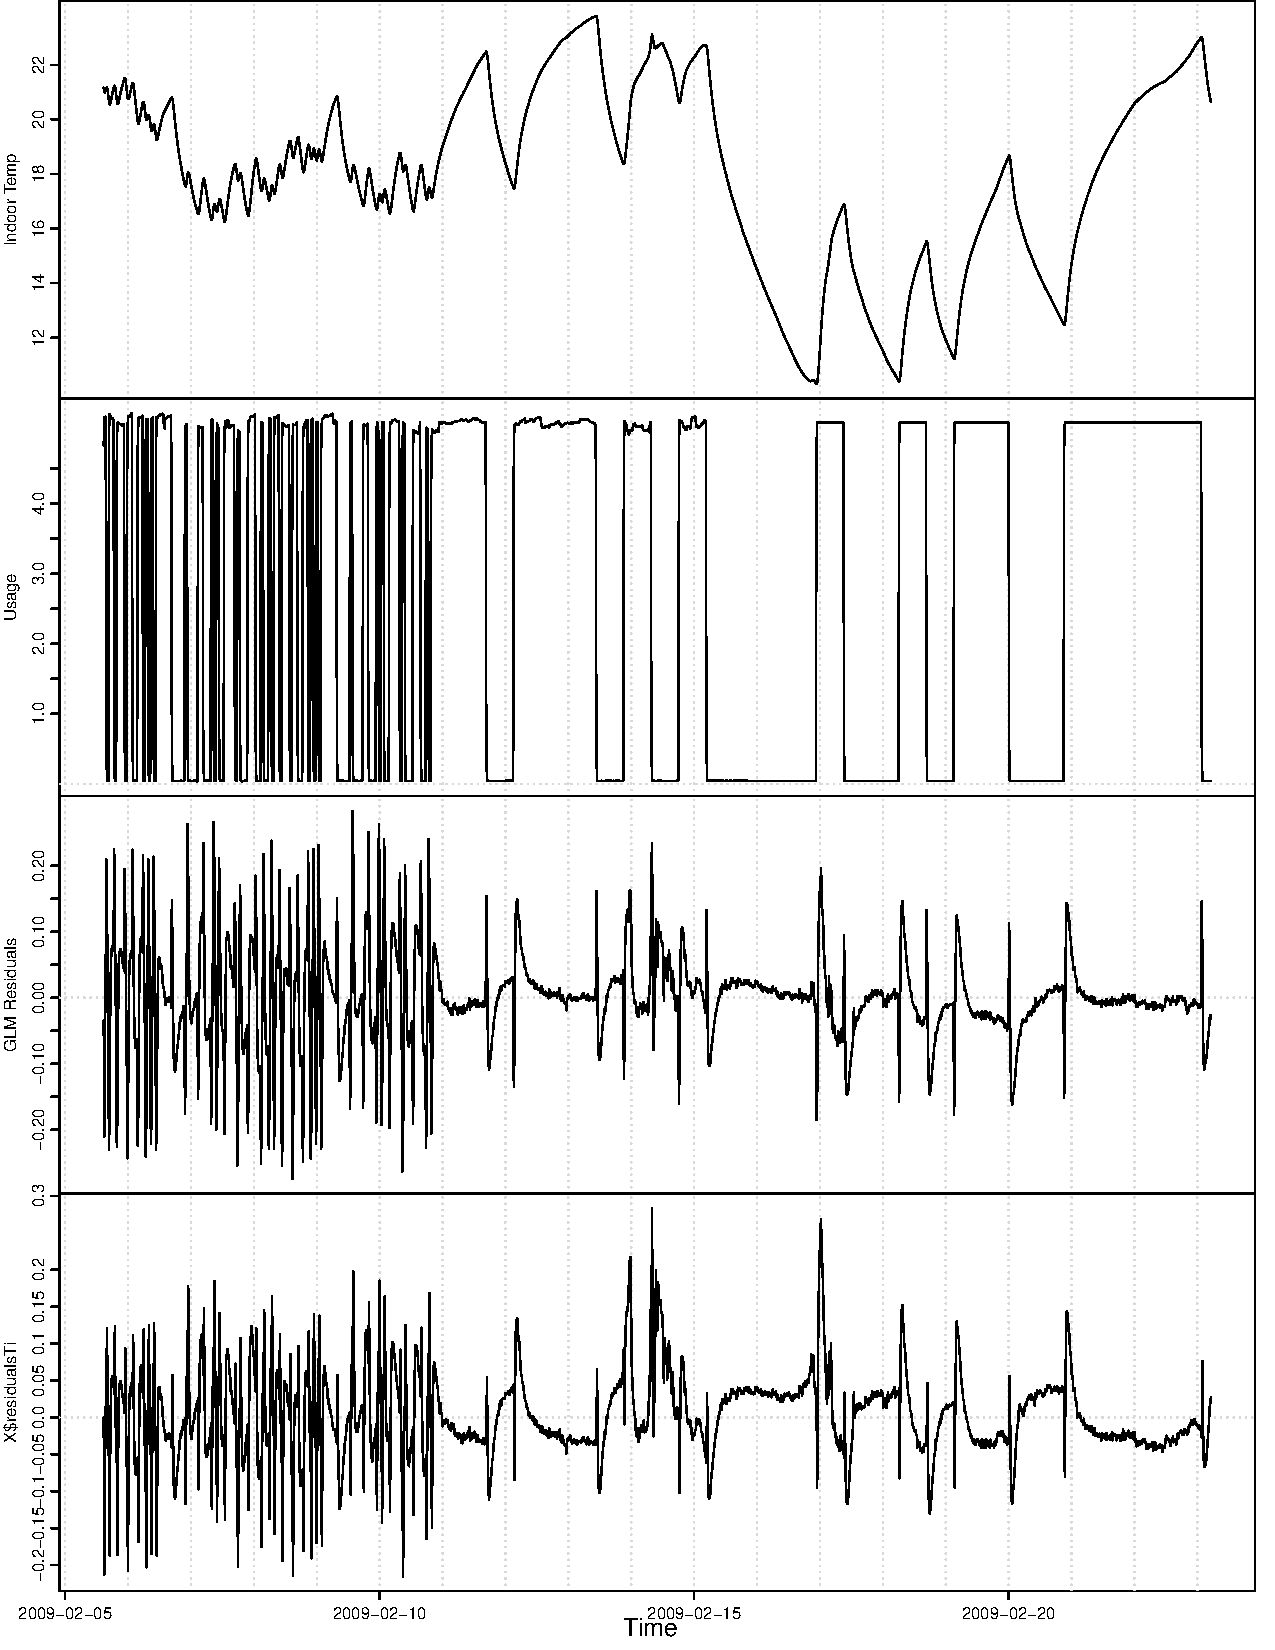
\includegraphics[height=3.6cm,width=3.2cm]{RplotResiduals}
    }\hspace{.7cm}
    \centering
     \subfloat[House 2470. $T_a$, $T_i$, dc]{
        \label{fig:subfig1}
        %\subcaption{House 2470: $T_a$,$T_i$ \& $\dc$}
        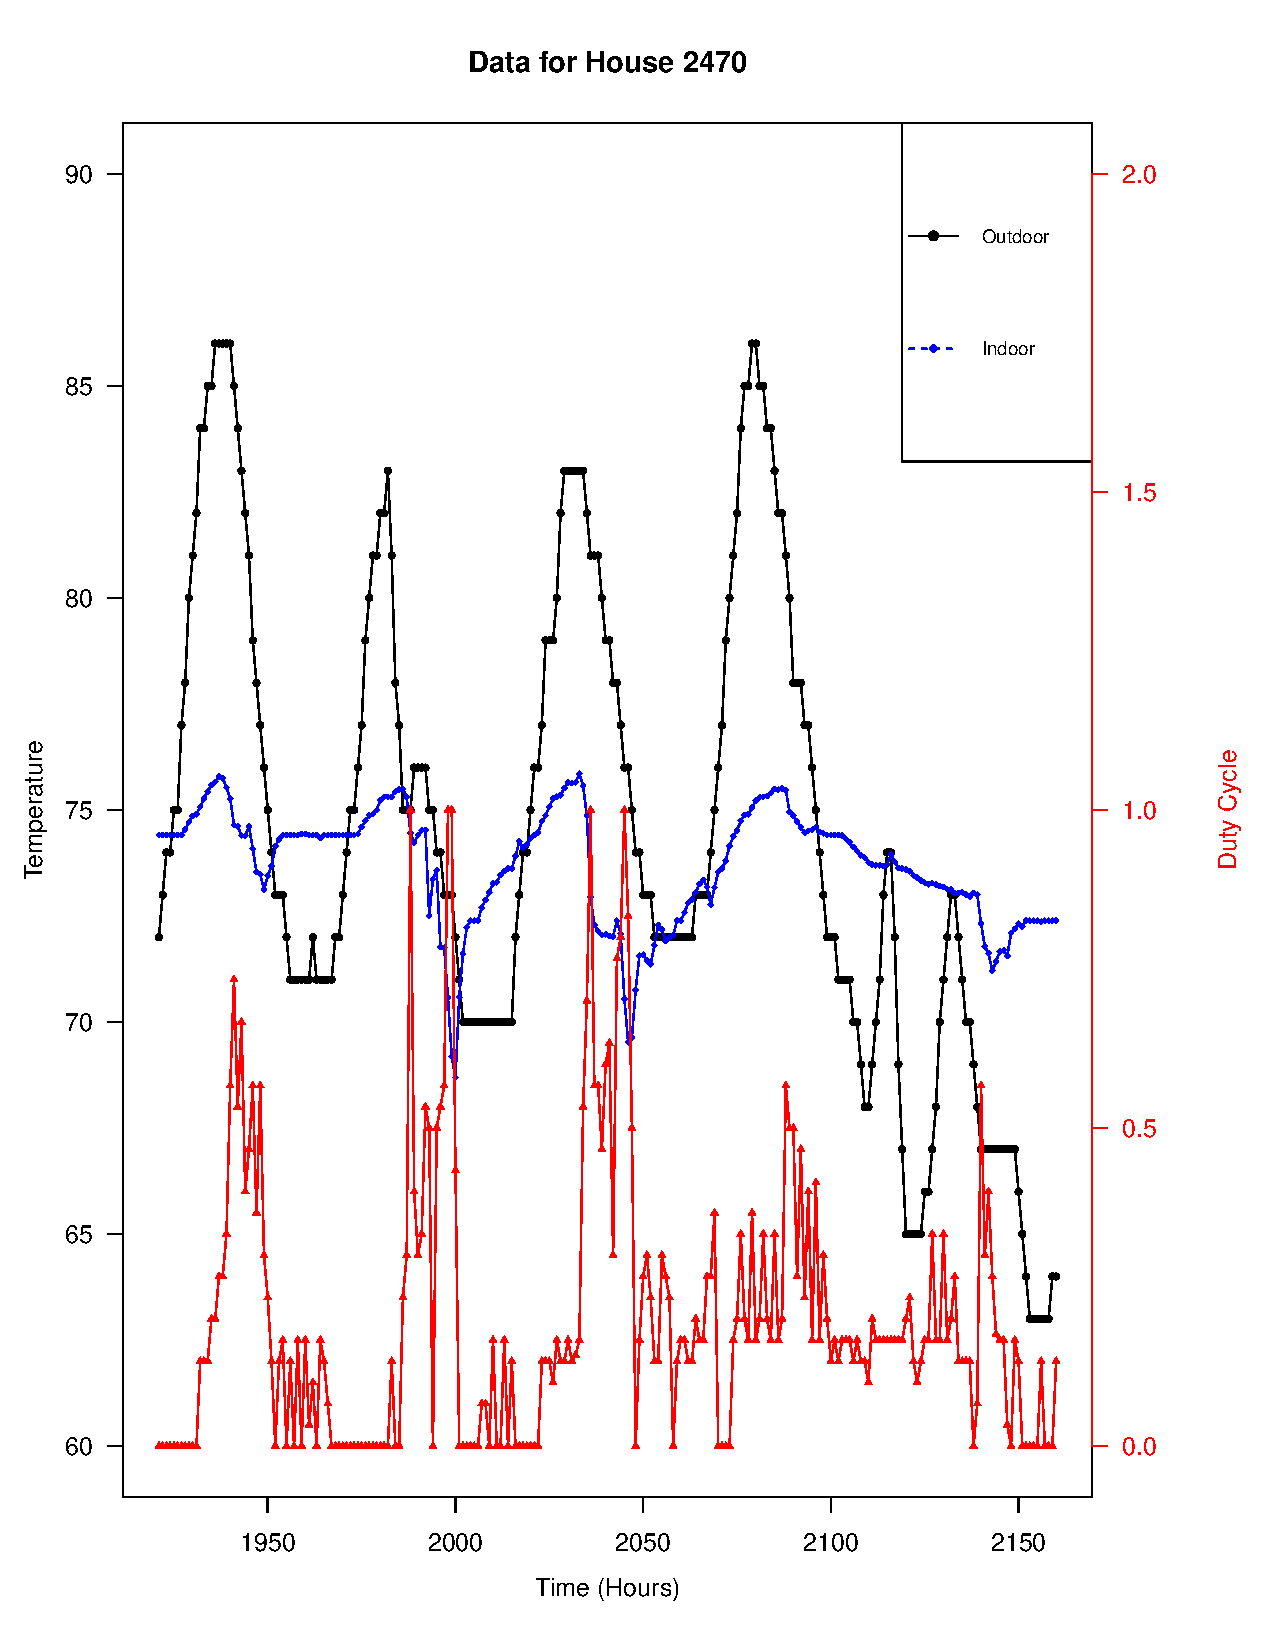
\includegraphics[height=4cm,width=4cm]{house2470}
    }
     \subfloat[ACF for a single day House 2470.]{
        \label{fig:subfig2}
       % \subcaption{ACF for a single day House 2470}
        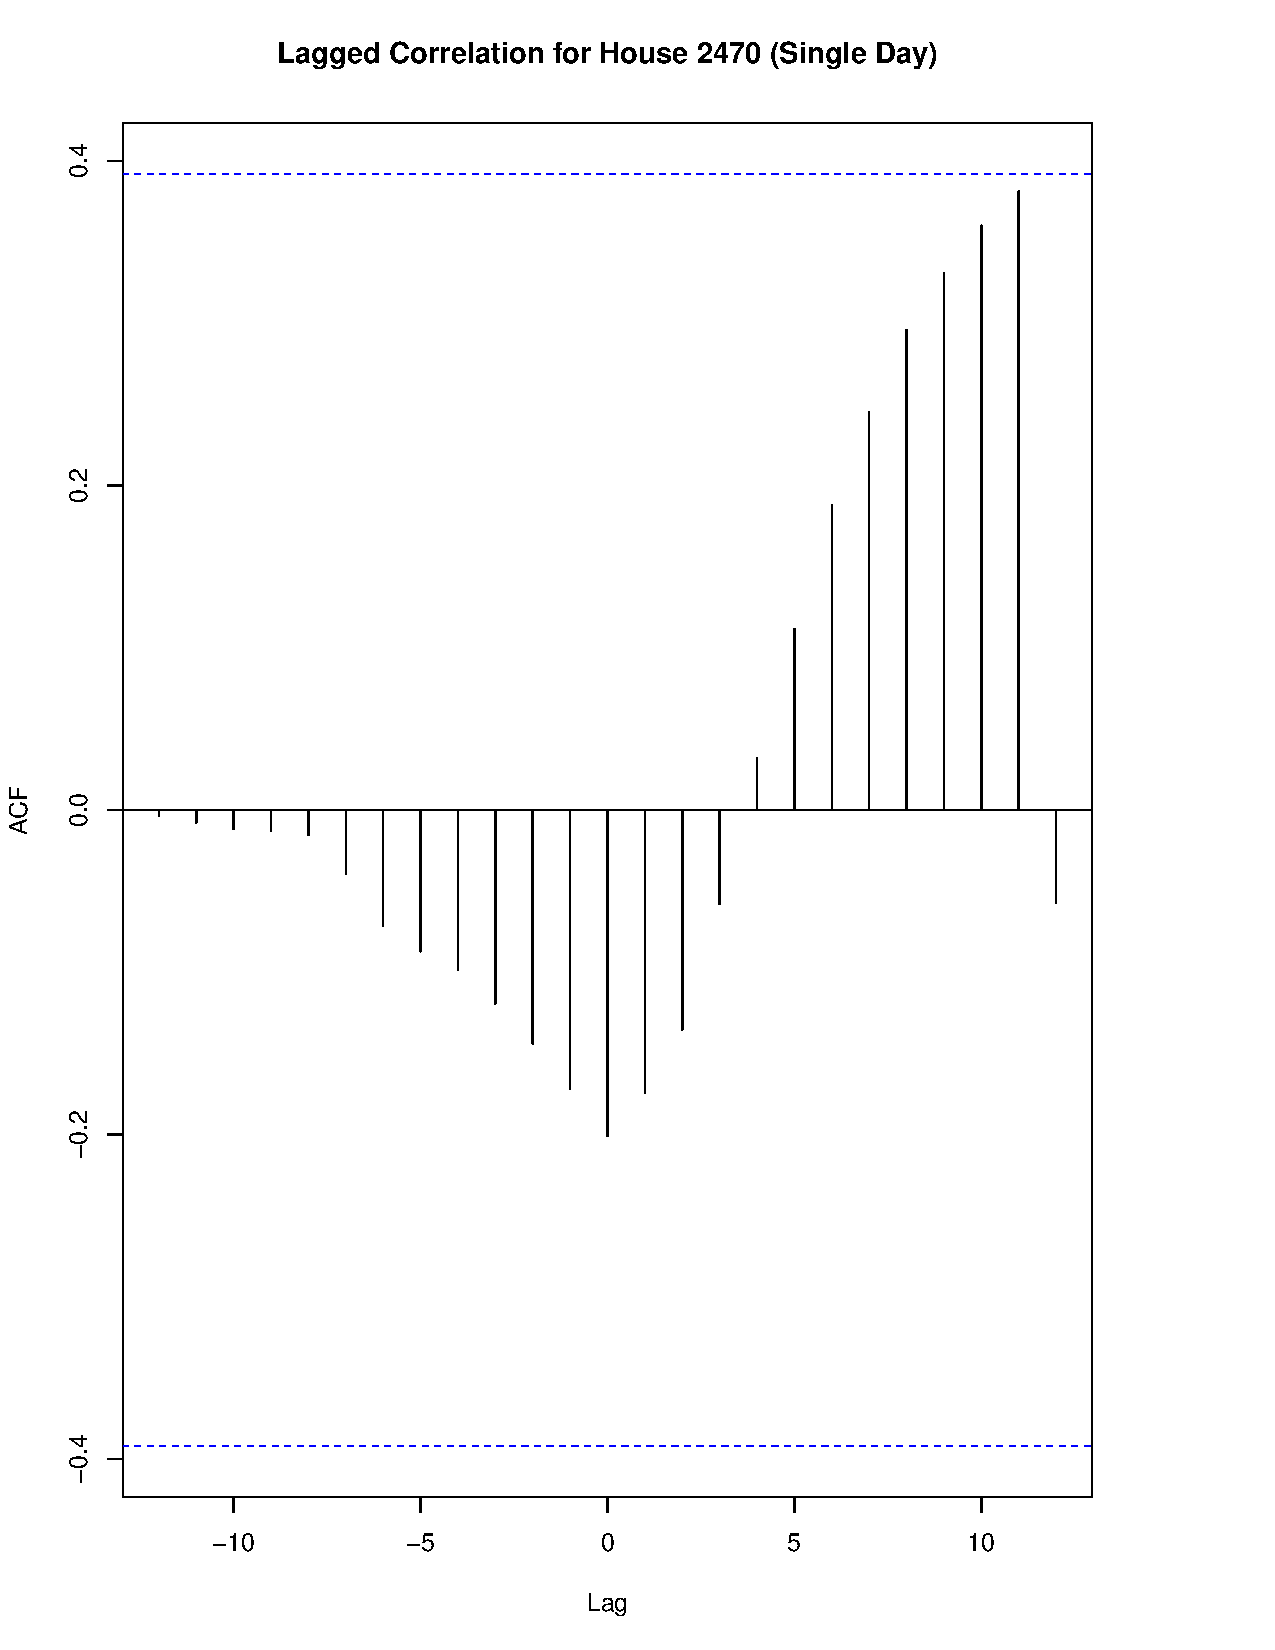
\includegraphics[height=4cm,width=4cm]{CCF2470}
    }
     \subfloat[House 410. $T_a$,$T_i$, AC, Heater]{
        \label{fig:subfig1}
       % \subcaption{House 1507. $T_a$,$T_i$, $\dc$}
        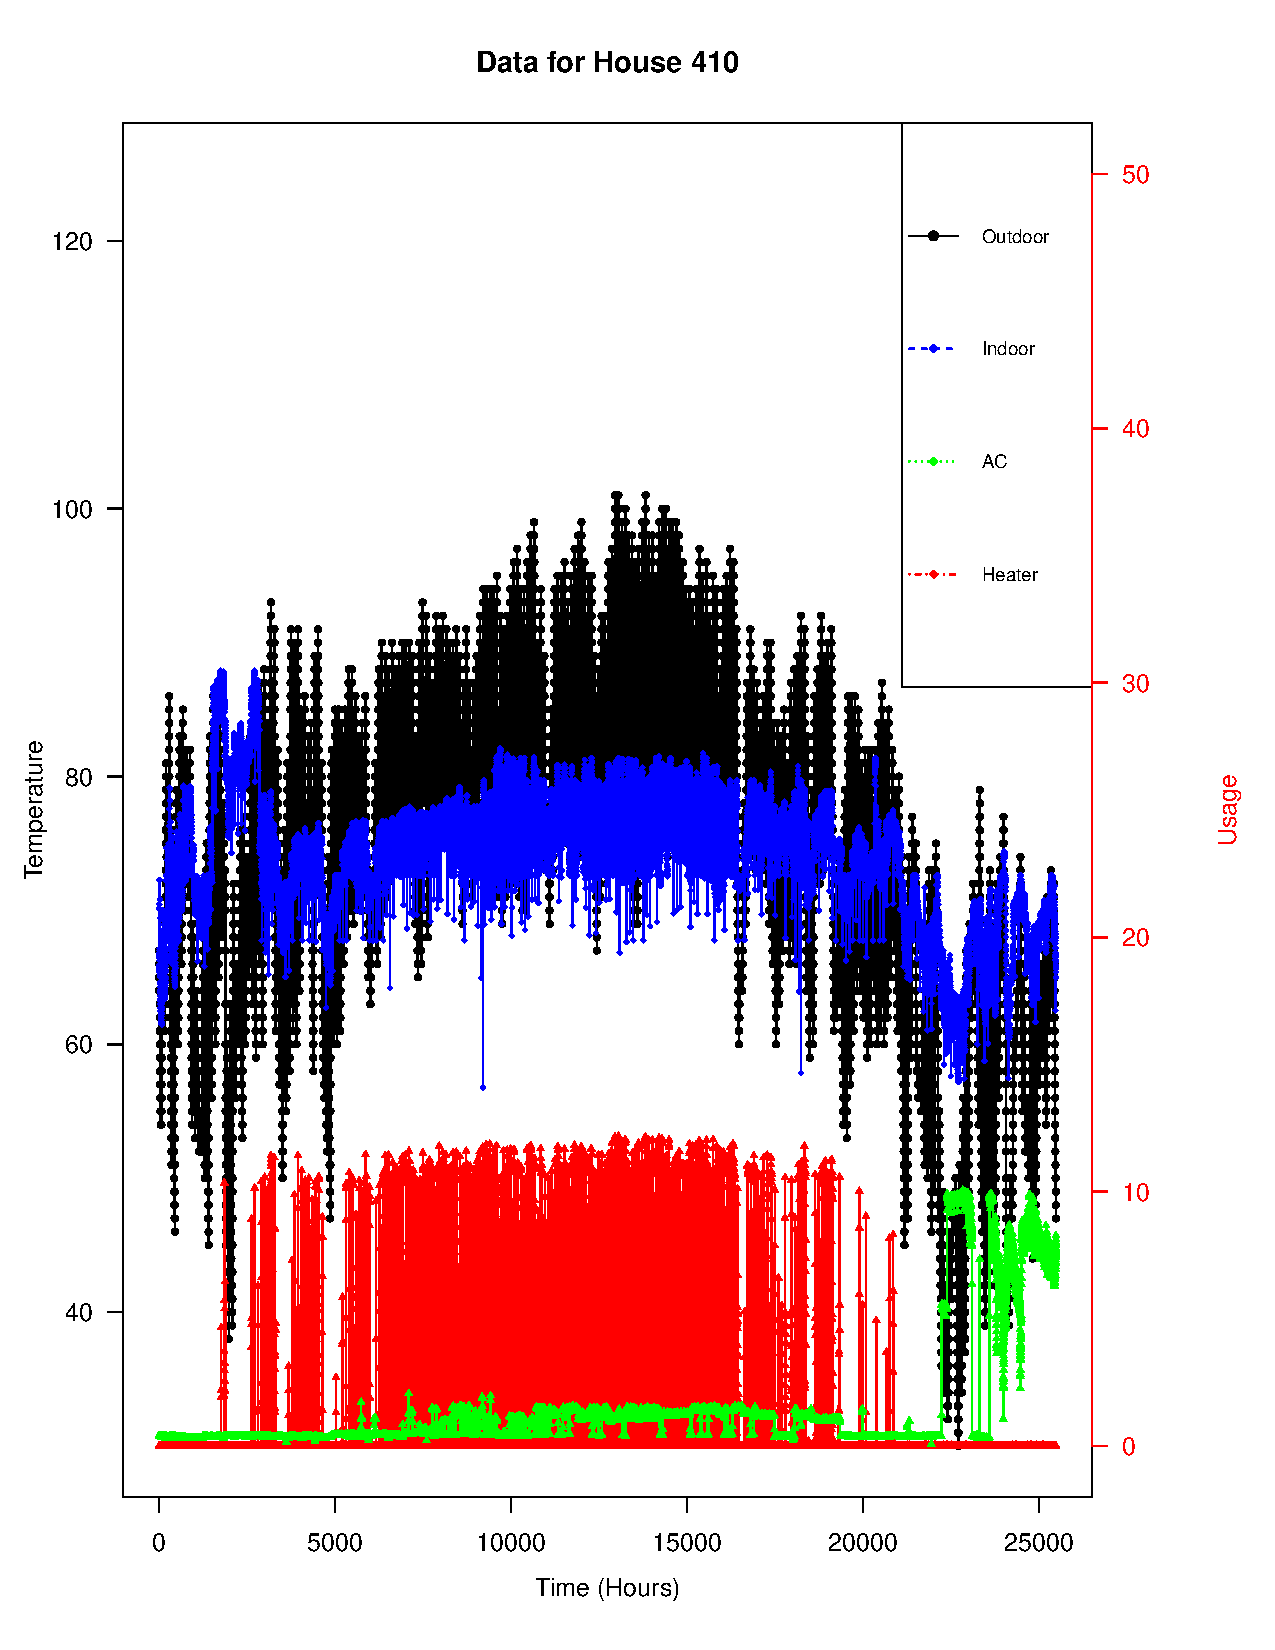
\includegraphics[height=4cm,width=4cm]{House410}
    }
    \caption{Sample Dataset of two homes}
    \label{fig:subfig}
\end{figure*}

	\input{Thermostats}
	

\subsection{IR Based Building characteristics}
\label{sec:IRLeak}

\indent After the identifying the potentially wasteful homes, we address the problem of detecting leakages and develop more detailed heat dynamics models of the homes. We compare two different datasets - one is the individual room-wise temperature data and the other is an image sensing unit using IR camera. 

\subsubsection{\textbf{Individual Roomwise Data for Modeling Heat Dynamics:}}

\indent We have setup temperature and humidity sensors in different parts of the house and have a NEST thermostat installed. The temperatures from different parts of the house is shown in Figure~\ref{fig:Sens}. It can be seen that different parts if the house has different dynamics of temperature. This is dependent on a number of factors like exposure to sun, local heaters being used. The objective here is to get a detailed model of the house in terms of individual room-wise parameter identification considering local factors. This in turn can help us isolate the leakages or poor thermal capacity or even the  

 
 
\subsubsection{\textbf{Imaging Device}}
 

The physical component of the thermal imaging system is a custom-created imaging device as pictured in Figure~\ref{tis:imp:ex}. Our prototypes are built from a Raspberry Pi Zero, a Raspberry Pi Camera Module, and a low-resolution IR camera, powered by a $5V$ battery, rotating on a DC motor, in a 3D printed housing. This sensor's purpose is to collect data from which to create a longitudinal thermal
map of a room and from which to detect the variations representing leakages and other energy waste.

There are two cameras in the imaging device. The IR camera is Melexis MLX90621~\cite{MLX}, which is a low resolution ($16\times$) and low power consumption of $<9mA$ when active and $<7\mu A$ otherwise. It can detect ambient temperature between  -40$^{\circ}$C  and 85 $^{\circ}$C  and object temperatures between  -50$^{\circ}$C  and  300$^{\circ}$C  with a resolution of  0.02$^{\circ}$C. The Raspberry Pi Camera Module~\cite{picam} is a RGB camera and collects images at $720\times480$ resolution. The 3D printed housing holds the cameras in a consistent relative position and orientation. The Raspberry Pi Zero controls the device and rotates the sensor unit (at 15min-1hour interval as per setting) for a number of steps sufficient to rotate at
least  360$^{\circ}$C. For every step, the Pi collects a simultaneous image from each camera. After the batch of rotations completes, the imaging device uploads the collected images to a server for processing.



%\textsc{\begin{figure}[t!]
%\begin{center}
%	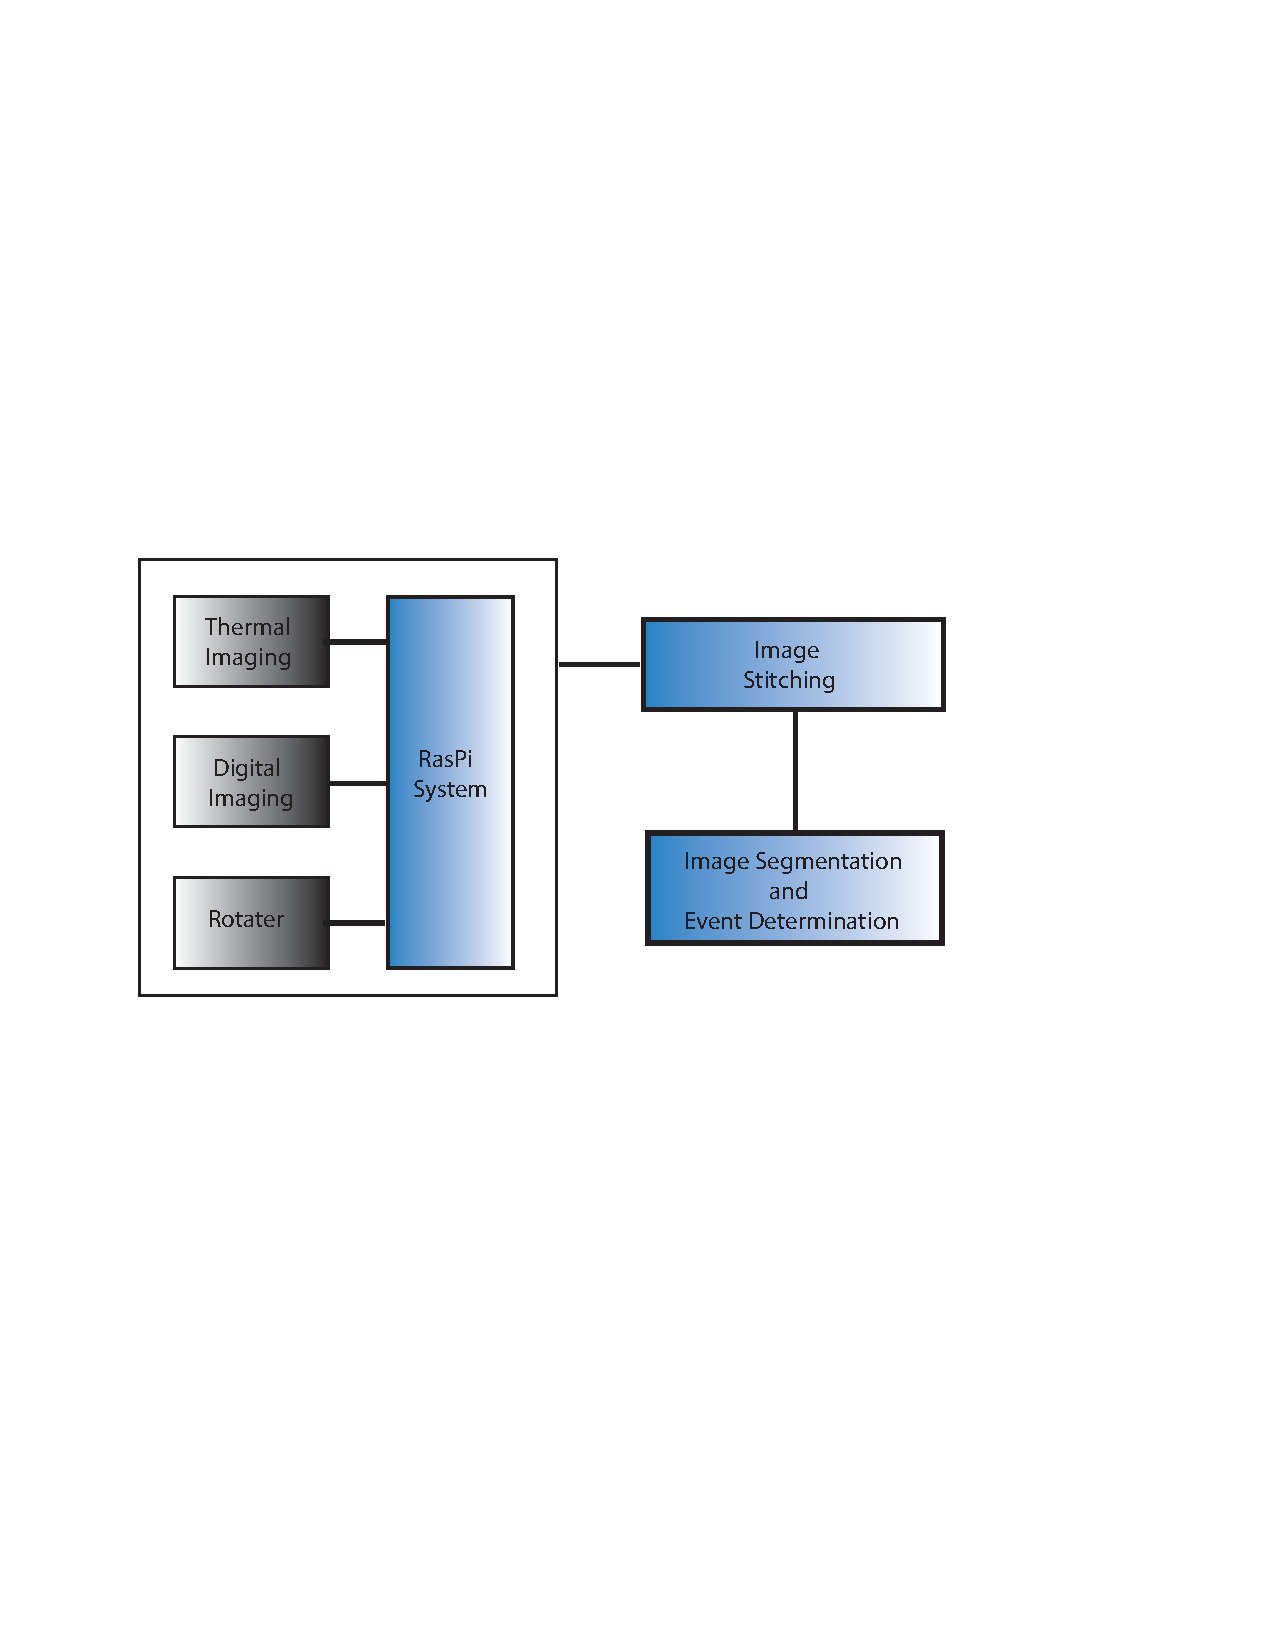
\includegraphics[width=3.5in]{figs/SystemArch.pdf}
%\end{center}
%  \caption{Thermal Imaging System Block Diagram}
%  \label{fig:Overview}
%\end{figure}}

	
\begin{figure}[h]
 \centering
    \subfloat[Imaging Device]{
      \label{tis:imp:ex}
        %\subcaption{House 2470: $T_a$,$T_i$ \& $\dc$}
        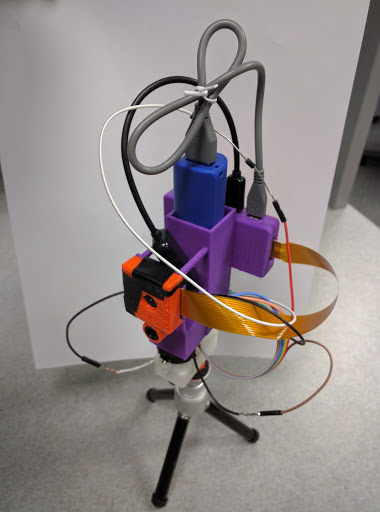
\includegraphics[height=.2\textheight,width=.15\textwidth,keepaspectratio]{CameraModule.jpg}
    }
       \centering
    \subfloat[Room-wise Temperature Sensor Data]{
      \label{fig:Sens}
        %\subcaption{House 2470: $T_a$,$T_i$ \& $\dc$}
        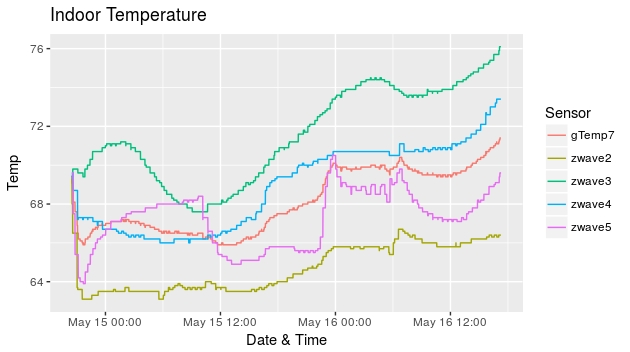
\includegraphics[height=6cm,width=.35\textwidth,keepaspectratio]{Temp.jpeg}
    }
    \caption{Imaging Device and Room-wise Temperature Data}
\end{figure}

\subsubsection{\textbf{Image Processing}}
 \indent On the image processing server, we use the RGB and IR image sets to generate a unified thermal map of the room. The first image processing step uses OpenCV to generate a panorama from the RGB images and record the homography matrices used for those image transformations. This process allows us to avoid the need for a heavier, more expensive stepper motor, because those homography matrices encode the relationships between sequential images. The second step uses those  matrices to produce an IR panorama of the room. The 3D printed housing of the imaging device maintains a fixed relationship between the positions and perspectives of the two cameras in each prototype. We calculate the mapping between the cameras once and, at processing time, use this transformation in addition to the homographies calculated in the RGB stitching process. Thus, we map each IR image on to its corresponding RGB image, then stitch those transformed IR images to create an IR panorama of the room.

\indent We propose to use the IR camera in tandem with a digital camera to detect and appropriately map the heatmap's points of interest in contrast to the presence of buildings air leakages, heat dissipation associated with different objects and appliances while achieving high precision and detection accuracy. While the specific color codes of heatmaps help detect the moderate, extreme or regular hot and cold surfaces, augmenting this with digital images helps detect any unusual usage behaviors, and operating conditions of everyday appliances in a smart home environment. For example, if a room has multiple windows and doors with air leakages or multiple similar small to medium load appliances, solely the heatmaps may not provide the home owners the adequate information as needed to detect any abnormal energy usage. While the IR camera albeit helps detect the region of interest but fails to provide the detailed identifications of the similar type of objects and appliances.

 
\indent We employ the digital stitching procedure~\cite{Stitch} to create the thermal panorama. We first stitch the digital images and maintain the respective control points for the stitching procedure which we reemploy to process the stitched thermal image generation. Next we augment the digital image in the background of the stitched thermal image based on the respective control points. We use a hybrid image construction methodology where the mask image or the thermal image is passed through a low pass filter and the digital image is passed through a high frequency filter to construct the digital image augmented heatmaps. We then apply a image segmentation algorithm to determine the different heatzone clusters in the stitched image. The temperature of each cluster is them compared with entries in a lookup table to determine the state of a specific appliance.  
 
\subsubsection{\textbf{Initial Image Analytics}}

There are three possible types of thermal regions in an image - background, cold region and hot region. The image that needs to be segmented is the stitched IR image and the objective is to create a thermal mask which separates the hot and cold regions from the background. Since the thermal image is being used for segmentation, the results are subject to the choice of color palette and range selection.  We ensure that the background has darker tones than the hot or cold surfaces which helps achieve the desired segmentation after image binarization using Otsu's method~\cite{OTSU}. We apply a 7$\times$7 neighborhood 2-D median filter to eliminate small blobs and isolate the few major thermal zones. Initial experiment suggested that the it is easy to detect human presence and objects as long as the wall temperature do not mask them. In Figure~\ref{fig:IR}, shows two sample stitched images during different time duration. It can be seen that there is a slight cool area detected near the window given in a deeper shade of blue. 

\begin{figure}[t]
 \centering
    \subfloat[Sample 1]{
      \label{fig:IR1}
        %\subcaption{House 2470: $T_a$,$T_i$ \& $\dc$}
        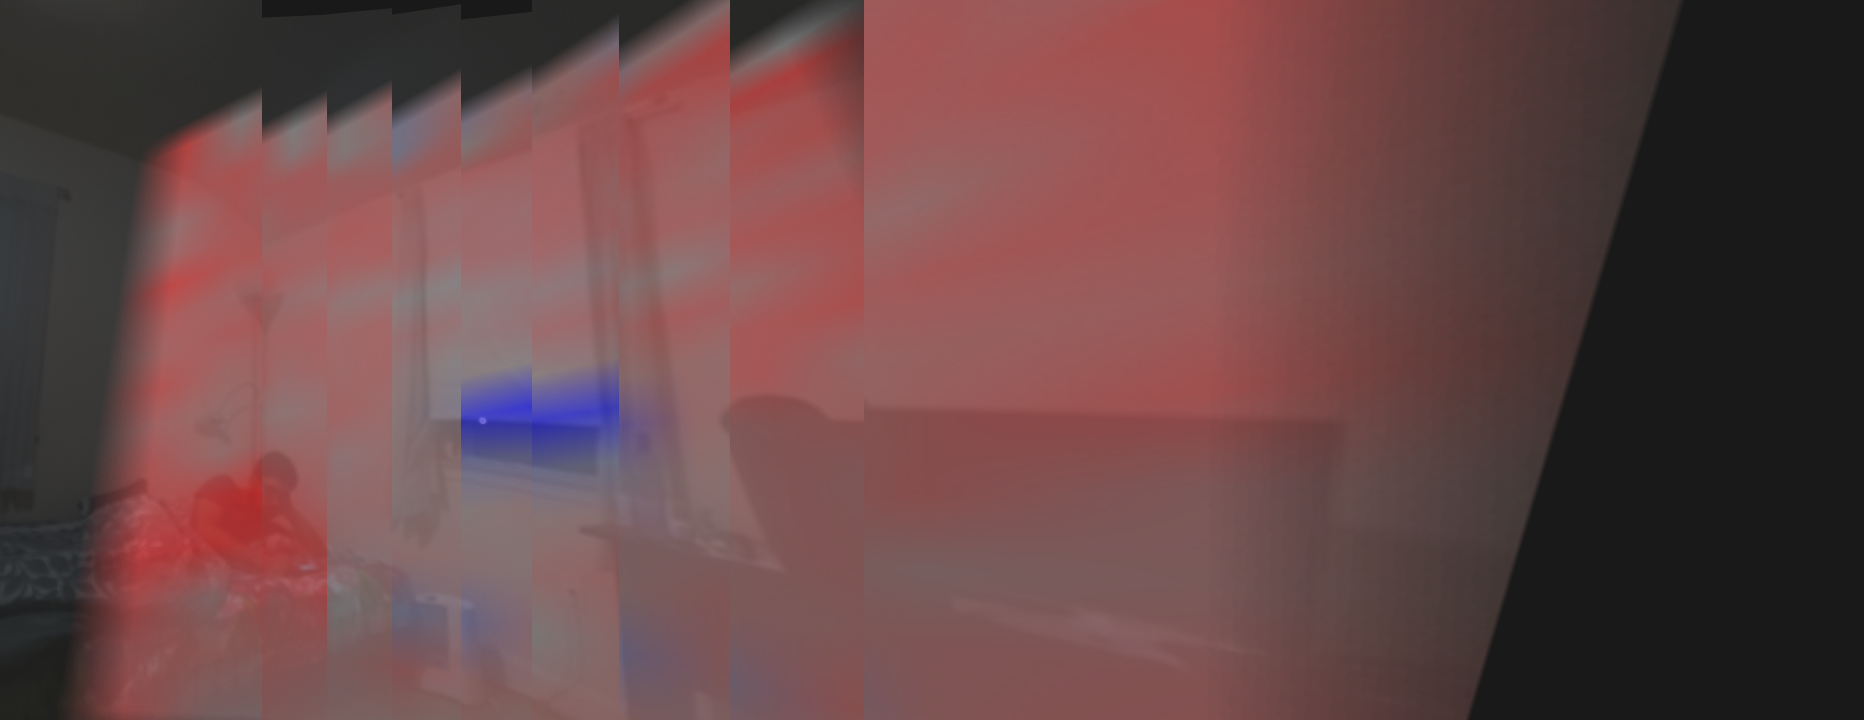
\includegraphics[height= 2cm,width=4cm]{overlay1}
    }
       \centering
    \subfloat[Sample 2]{
      \label{fig:IR2}
        %\subcaption{House 2470: $T_a$,$T_i$ \& $\dc$}
        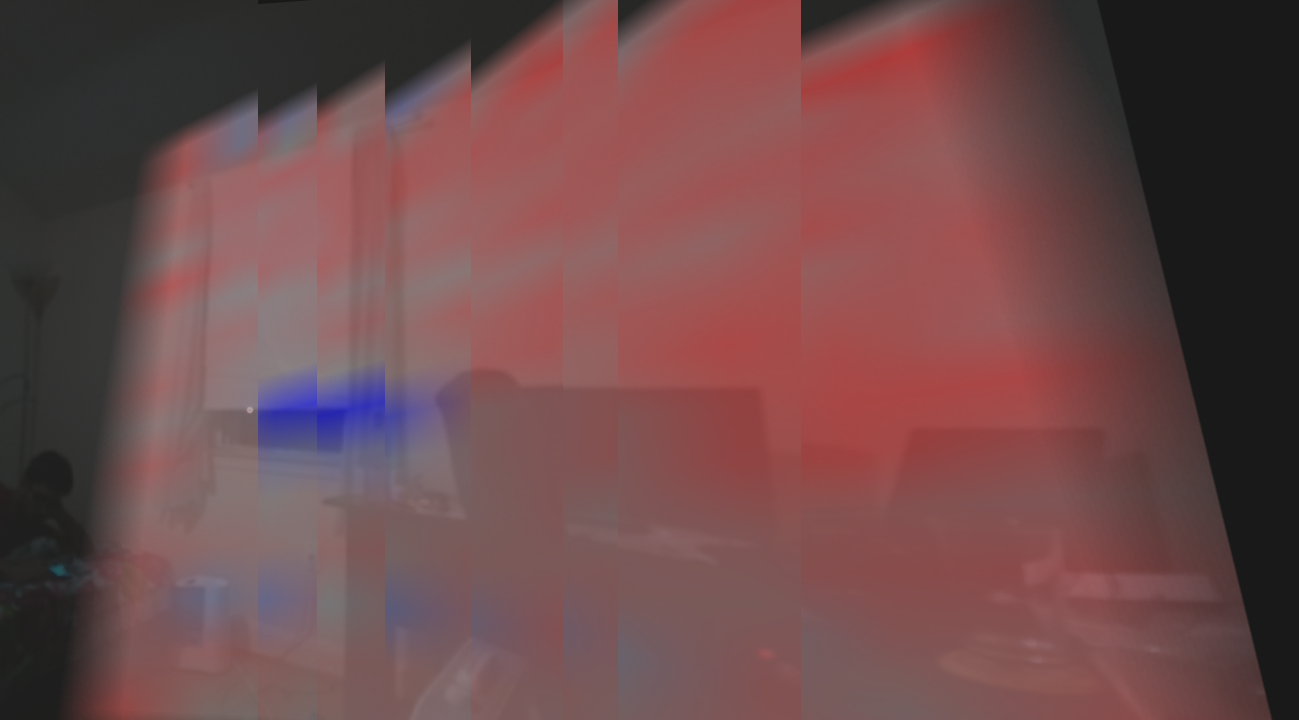
\includegraphics[height=2cm,width=4cm]{overlay2}
    }
    \caption{Overlapped Room Image and IR image}
    \label{fig:IR}
\end{figure}

\indent The challenges in stitching mainly stem from our simple approach. Better image stitching can solve the problem. Alternatively, rotating the unit on a stepper motor, instead of DC motor, can be another solution which can up the unit price by \$8. We're doing feature-detection based stitching, which has a lot more difficulty with close-up objects and with blank, featureless walls and the unit positioning is another factor. Ideally keeping the unit centered in the room may solve the problem however that can cause logistical problems.  
	\input{Conclusion}

\end{document}